\documentclass[a4paper, 12pt]{report}

% Packages
\usepackage[utf8]{inputenc}
\usepackage[T1]{fontenc}
\usepackage[french]{babel}
\usepackage{graphicx}
\usepackage{float}
\usepackage{hyperref}
\usepackage{fancyhdr}
\usepackage{titlesec}
\usepackage{lipsum}

% Mise en page
\pagestyle{fancy}
\fancyhf{}
\setlength{\headheight}{15pt}
\renewcommand{\headrulewidth}{0.5pt}
\renewcommand{\footrulewidth}{0pt}
\lhead{\leftmark}
\rhead{\thepage}
\renewcommand{\chaptermark}[1]{\markboth{\MakeUppercase{#1}}{}}
\titleformat{\chapter}[display]{\normalfont\huge\bfseries}{\chaptertitlename\ \thechapter}{20pt}{\Huge}
\graphicspath{ {./images/} }

% Informations du document
\title{Test Rapport de projet d'électronique pour système embarqué}
\author{Simon GIRARD - Dimitri TIMOZ - Mathis SAUNIER - Alix ANNERAUD}
\date{\today}

\begin{document}

% Page de garde
\begin{titlepage}
\maketitle{}
\end{titlepage}

% Table des matières
\tableofcontents

% Chapitres
% An introduction with the project objectives
\chapter{Introduction}
\lipsum[1-2]
% 
\chapter{Contexte}
\lipsum[3-4]

\chapter{Conception}

% A complete fritzing circuit with all the wiring of the different sensors, actuators and components for display
% + A detailed explanation of your wiring choices as well as any additional technical choices (power, use of resistors, diodes, etc.)
% + A detailed explanation of the chosen components role and operating principle
\section{Electronique}
\subsection{Choix des composants}
\subsection{Cablâge des composants}
\subsection{Schéma EasyEDA}
% A detailed section of your code: approach, structure, etc.
\section{Code}
\subsection{Architecture du programme}
\subsection{Développement des fonctions métiers du robot}
% Là je sais pas mais on pourrait faire les fonctions des roues, l'algo pour le chemin, le multi threading, le code pour le son ...

\subsection{Développement de l'interface de contrôle}
% Ici aussi on pourrait détailler succintement avec la communication serveur/robot, la manette, la soundboard et les réglages de vitesse du robot + l'affichage au besoin des logs, de la caméra etc ...
\section{Mécanique}
\subsection{Choix de la taille des roues}
\subsection{Emplacement des roues et des capteurs}

% A section with detailing each member’s taks in the project + l'organisation interne
\chapter{Méthodologie}
\lipsum[5-6]

\chapter{Résultats}
\lipsum[7-8]
\section{Difficultés rencontrées}
\subsection{Problèmes de son}
Au tout début du projet, durant la conception de notre robot, l'idée d'ajouter un haut-parleur nous est rapidement venu. Le concept était très simple : utiliser le port jack intégré à notre Raspeberry Pi pour émettre un son qui sera ensuite amplifié avant d'être émis par un haut-parleur.
En fin de compte, cette fonctionnalité a été un vrai challenge à ajouter sur notre robot et c'est pour cete raison que nous y dédions une sous-partie du rapport. Nous détaillerons toutes les solutions essayées ainsi que la solution finalement retenue.
\\
La première solution censée apporter le son à notre robot a été le module d'amplification suivant : 386AMP from DFRobot
\\
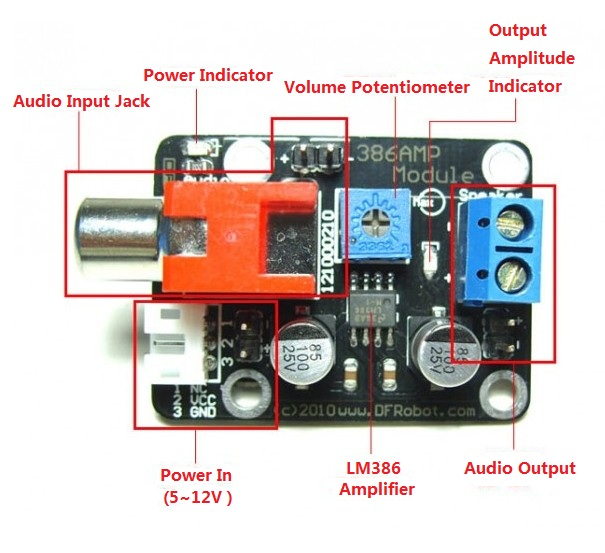
\includegraphics[scale=0.5]{386AMP.jpg}
\centering
\\
Une première difficulté est survenue. Il nous fallait un câble jack 3.5 vers RCA afin de pouvoir utiliser le module d'amplification sur lequel pouvait ensuite être aisément branché un haut-parleur. Étant donné que le laboratoire d'électronique ne possédait pas ce type de câble,
nous avons fini par trouver le matériel nécessaire chez nous. Ainsi, nous avons pu faire les premiers tests du module avec des téléphones. Ces derniers étant concluants, nous avons recherché les commandes nécessaires à la lecture d'un audio sur Raspeberry. Nous utilisons donc 3 fonctions systèmes
de la Raspeberry.
\begin{itemize}
    \item system("amixer -q set PCM,0 unmute"); permet de s'assurer que le son de la Raspeberry est actif
    \item system("mpg321 -q assets/" + filename + " \&"); permet de lancer, en processus d'arrière plan, l'audio désigné par la variable filename
    \item system("pkill -9 mpg321"); permet d'arrêtter le processus qui joue la musique en cours
\end{itemize}

\subsection{Échec des capteurs QTR}
\subsection{Tentative d'algorithme suiveur de ligne PID}
\subsection{Retours d'expériences}
% Partie dans laquelle on revient sur ces difficultés, on essaie de les raisonner
% (leur trouver une raison) et faire comme si le projet avait été une source incroyable d'apprentissage pour nous
\section{Les capacités du robot}

\chapter{Conclusion}
\lipsum[9-10]

% Bibliographie
\begin{thebibliography}{9}
\bibitem{latexcompanion} 
Michel Goossens, Frank Mittelbach, and Alexander Samarin. 
\textit{The \LaTeX\ Companion}. 
Addison-Wesley, Reading, Massachusetts, 1993.

\bibitem{einstein} 
Albert Einstein. 
\textit{Zur Elektrodynamik bewegter K{\"o}rper}. (German) 
[\textit{On the electrodynamics of moving bodies}]. 
Annalen der Physik, 322(10):891–921, 1905.

\bibitem{knuthwebsite} 
Knuth: Computers and Typesetting,
\\\texttt{http://www-cs-faculty.stanford.edu/\~{}uno/abcde.html}
\end{thebibliography}

\end{document}
